Aufgrund des in \autoref{tab:bewertungsmatrix-echtzeit} durchgeführten Vergleiches, den Kinesis (Data Streams und Analytics) anführte, wird im Folgenden die Referenzarchitektur für die Echtzeitverarbeitung mit Kinesis Data Streams und Analytics entworfen. Diese Referenzarchitektur entspricht dem in \autoref{chap:bestehende_ras} vorgestellten Konzept einer $\kappa$-Architektur. Zuerst wird Folgend die Datenverarbeitungssequenz der Referenzarchitektur gezeigt. Folgend, als darauf aufbauende Dekomposition wird die Verteilungssicht gezeigt. Die Verteilungssicht wird detailliert durch die Bausteinsicht. Folgend werden die Anforderungen der Stakeholder addressiert. Um einen guten Betrieb der instanziierten Architekturen sicherzustellen, wird folgend ein Monitoringkonzept vorgestellt. Abschliessend wird diverses Know-how als Sammlung der abseits von den Dekompositionssichten zu beachtenden Funktionsweisen der Diensten dargestellt.

Die Dekompositionssichten enthalten durch \textbf{VP} gekennzeichnete Variationspunkte. Gemeinsame Variationspunkte zwischen den Dekompositionssichten oder den Referenzarchitekturen bekommen den Buchstaben G und eine fortlaufende Nummer und werden nur einmal erklärt. Folgend wird auf die gemeinsamen Variationspunkte zurückverwiesen.

\subsection{Datenverarbeitungssequenz}
\autoref{abb:SequenceEchtzeitRAIngestion} und \autoref{abb:SequenceEchtzeitRAAnalysis} zeigen die durchlaufene Sequenz für eingehende Daten. \autoref{abb:SequenceEchtzeitRAIngestion} zeigt dabei speziell die initialer Übertragung via \ac{MQTT} an \AWSIOT{} Core. Es folgt die Übertragung an Kinesis Data Streams oder Kinesis Data Firehose, wie in \vpref{G1} beschrieben. Anschließend werden die Daten gepuffert an Kinesis Data Analytics gesendet. 

\begin{figure}[H]
\centering
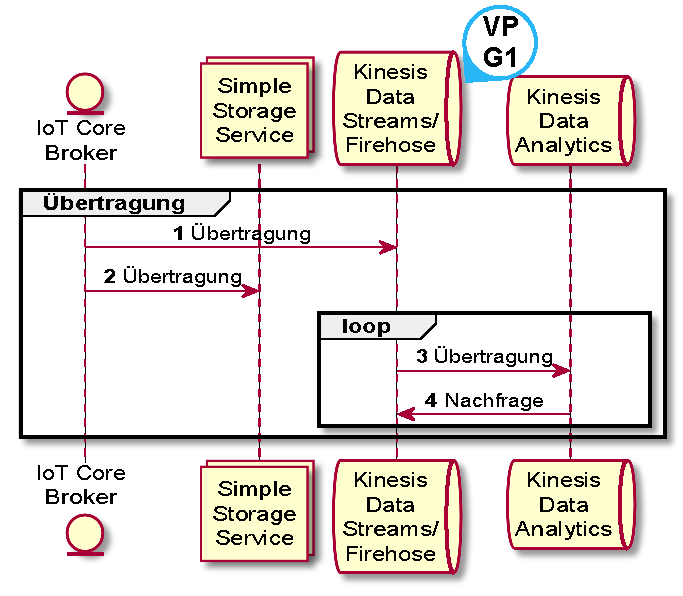
\includegraphics[height=0.4\textheight]{graphics/echtzeit-ra-ingestion.pdf}
\caption{Sequenzdiagramm Echtzeitreferenzarchitektur Dateneingang}
\label{abb:SequenceEchtzeitRAIngestion}
\end{figure}

\vp{G1}: Je nach Anforderung kann Kinesis Data Firehose oder Kinesis Data Streams verwendet werden. Während die höhere Abstraktion und das einfachere Abrechnungsmodell von Kinesis Data Firehose einen reduzierten Wartungsaufwand hat, bietet Kinesis Data Streams mehr Kontrolle über unterliegende Faktoren wie Datenaufbewahrung und Durchsatz. Kinesis Data Firehose benötigt zwingend ein \enquote{Delivery Ziel}. Dies kann beispielsweise ein \ac{S3}-Bucket, eine Redshift Datenbank oder eine Elasticsearch Datenbank sein. In diesem Fall wurde aus Kosten- und Umsetzungserwägungen ein \ac{S3}-Bucket gewählt.

In \autoref{abb:SequenceEchtzeitRAAnalysis} ist die auf die Datenübertragung folgende Analyse gezeigt. Kinesis Data Analytics führt dabei die Analyse durch und überträgt die Ergebnisse an Lambda. Nach Auslösung überträgt Lambda die Alarme an \ac{SNS}. QuickSight wird, wenn \vpref{G2} verwendet wird, zur Visualisierung analysierter und gespeicherter Rohdaten verwendet.

\begin{figure}[H]
\centering
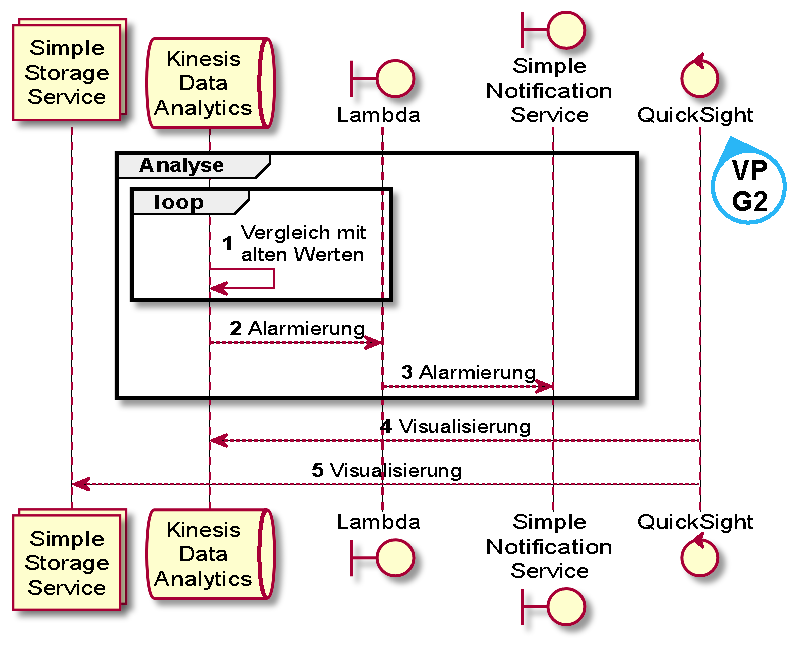
\includegraphics[height=0.43\textheight]{graphics/echtzeit-ra-analysis.pdf}
\caption{Sequenzdiagramm Echtzeitreferenzarchitektur Datenverarbeitung}
\label{abb:SequenceEchtzeitRAAnalysis}
\end{figure}

\vp{G2}: QuickSight als \ac{AWS} native Dashboardlösung ist gut geeignet, um schnell eine Übersicht der Datenanalysen von Kinesis Data Analytics zu bekommen. Alternativ können auch andere Visualisierungslösungen wie Tableau eingesetzt werden, welche gegebenenfalls jedoch keinen (vollen) Zugriff auf Kinesis Data Analytics haben. Ein weiterer managed Service, den \ac{AWS} für Dashboards anbietet, ist der Amazon Managed Service for Grafana, welcher das Open Source Visualisierungstool Grafana mit den \ac{AWS} eigenen Metriken integriert.\footcite[Vgl.][]{Dutt.2020} In diesem Fall kann der \ac{S3} Bucket verwendet werden, um Dashboards über die Rohdaten zu erstellen. 

\subsection{Verteilungssicht}
Folgend ist die Verteilungssicht der Echtzeitreferenzarchitektur gezeigt, als Dekomposition der Datenverarbeitungssequenz.
\begin{figure}[H]
\centering
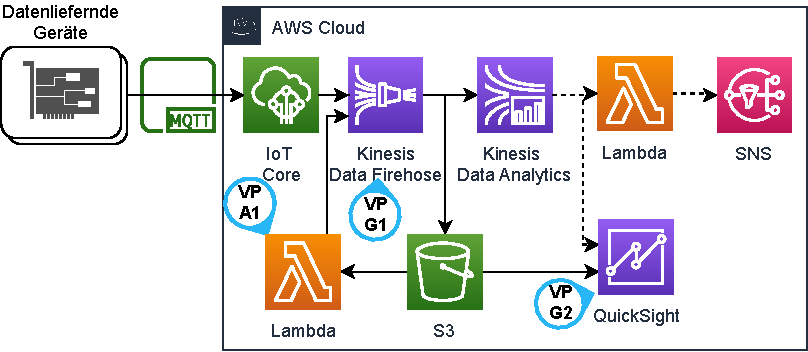
\includegraphics[width=\textwidth]{graphics/Echtzeit-RA-Overview-Firehose}
\caption{Verteilungssicht mit Data Firehose}
\label{abb:TopLevelEchtzeitRA}
\end{figure}

\textbf{Variationspunkte G1, G2}: Siehe oben: \vpref{G1}, \vpref{G2}

\vp{A1}: Sollte es nicht erforderlich sein, Daten erneut in Kinesis Data Firehose einzuspielen, kann auf die Lambdafunktion verzichtet werden. Diese liest, wenn manuell aktiviert, den \ac{S3}-Speicher ein und spielt die erfassten Nachrichten erneut in der selben Sequenz in Kinesis Data Firehose ein. Notwendig wird diese Lambda, wenn historische Daten mit abweichender Analyselogik analysiert werden sollen.

Im Folgenden wird die Verteilungssicht im zweiten Fall von \vpref{G1}, der Verwendung von Kinesis Data Streams gezeigt. Die Auswahl von Kinesis Data Streams ist insbesondere angezeigt, wenn die Nachrichten direkt aufbewahrt werden sollen und direkter Einfluss auf die Performance erwünscht ist.

\begin{figure}[H]
\centering
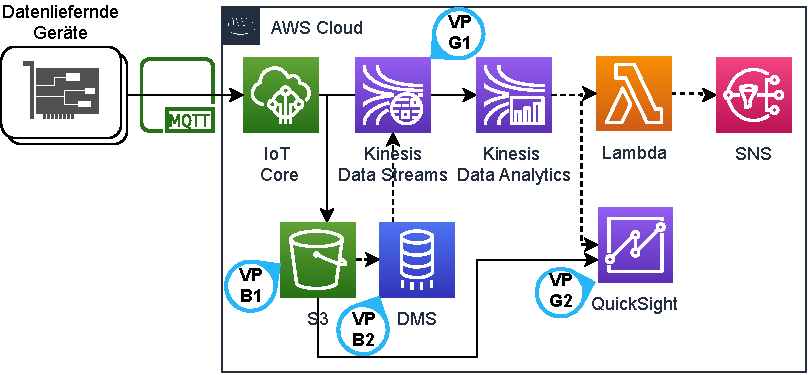
\includegraphics[width=\textwidth]{graphics/Echtzeit-RA-Overview.pdf}
\caption{Verteilungssicht mit Data Streams}
\label{abb:TopLevelEchtzeitRAStreams}
\end{figure}

\textbf{Variationspunkte G1, G2}: Siehe oben: \vpref{G1}, \vpref{G2}

\vp{B1}: Rohdaten in \ac{S3} zu speichern kann Sinn machen, um die Daten später noch einmal analysieren zu können. Nimmt man aber die Theorie der Datenhalbwertszeit zur Hilfe, macht es vielleicht Sinn, die Daten stattdessen maximal sieben 
Tage in Kinesis Data Streams zwischenzuspeichern und auf \ac{S3} zu verzichten. Mittels der erweiterten Aufbewahrung $\lbrack$\textit{Data Retention}$\rbrack$ können Analysen mehrfach im Fehlerfall angefordert werden. Da die Preise nach sieben Tagen Aufbewahrung ansteigen und für Aufbewahrung und Abruf doppelt abgerechnet wird, ist zu empfehlen, die Daten am Ende des siebten Tages zu verwerfen.\footcite[Vgl.][]{AmazonWebServicesInc..o.J.l} Dieser Variationspunkt ist abhängig vom \vpref{G1}, da Kinesis Data Firehose keine erweiterte Aufbewahrung unterstützt und die Daten in \ac{S3} abgelegt werden müssen.

\vp{B2}: \ac{DMS} ist in diesem Szenario dafür gedacht, einmal abgelegte Daten in S3 wieder in Kinesis Data Streams einspielen zu können. Je nach Szenario ist dies, wie bei \vpref{B1} schon erläutert, nicht notwendig.

\subsection{Bausteinsicht}
Unter Berücksichtigung von \vpref{G1} ergeben sich aus der Verteilungssicht zwei Bausteinsichten. Dies ist bedingt durch die sich ergebenden architekturellen Änderungen, beim Einsatz von Kinesis Data Streams oder Kinesis Data Firehose. Folgend wird zuerst Kinesis Data Firehose vorgestellt.

\begin{figure}[H]
\centering
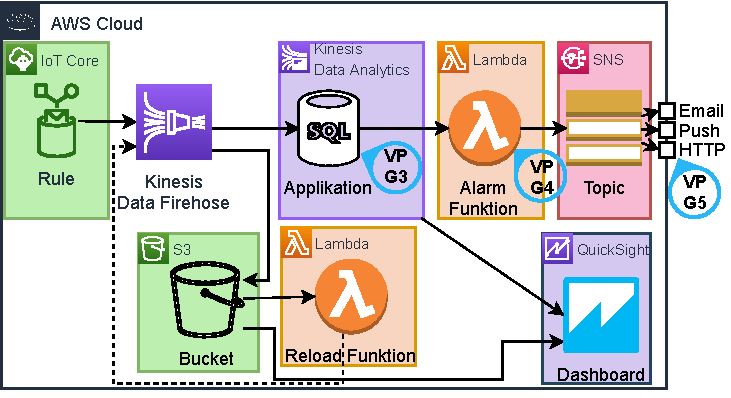
\includegraphics[width=\textwidth]{graphics/Echtzeit-RA-Elements-Firehose.pdf}
\caption{Bausteinsicht mit Data Firehose}
\label{abb:ElementeEchtzeitRA}
\end{figure}

\vp{G3}: Der \ac{SQL} Programmcode, der in Kinesis Data Analytics läuft, ist anzupassen. So sind Verarbeitungsfenster, Attributsnamen und aufgerufene Funktionen nach Anforderung zu ändern. Andernfalls kann auch die Funktionalität zur Ausführung eigenen Codes via Apache Flink in Kinesis Data Analytics genutzt werden (dies erlaubt Ausführung von Java, Scala, Python). Dies ist angezeigt, wenn der \ac{SQL}-Dialekt die gewünschten Auswertungen nicht unterstützt, oder eine eigene Implementierung vorgesehen ist.

\vp{G4}: Aufgrund der Notwendigkeit einer Lambda Funktion, um Alarme zu versenden, kann der Code selbst gestaltet werden. Wichtig ist dabei, dass Kinesis Data Analytics die Zustellung von Datensätzen wiederholt, wenn die Lambdafunktion als Rückgabewert ein Array mit den Ids und dem Status wie folgt zurückgibt: \mintinline[breaklines]{json}{[{"recordId": "<ID>", "result": "DeliveryFailed"}]}.\footcite[Vgl.][]{AmazonWebServicesInc..o.J.ay} Die übermittelten Alarme lassen dabei Möglichkeit zur Anpassung. So kann neben dem Titel der Nachricht auch der eigentliche Inhalt angepasst werden. Beispielhaft ist in \anhangref{anhang:echtzeit-codesample} gezeigt, wie eine in JavaScript geschriebene Lambdafunktion aussehen könnte, die via Kinesis Data Analytics angesteuert wird. Diese Funktion gibt selbstständig fehlerhafte Nachrichten zur Wiederverarbeitung an Kinesis Data Analytics zurück, versendet \ac{SNS} Alarme und kann via \ac{MQTT} eine Shutdown Nachricht an das Gerät übermitteln.

\vp{G5}: \ac{SNS} unterstützt mehrere Protokolle für die Übermittlung von Nachrichten. Es können HTTP Webhooks genauso wie mobile Pushbenachrichtigungen oder auch Emails versendet werden. Welches Protokoll mit welchem Verteiler zu wählen ist, muss im \ac{SNS} Topic eingestellt werden. Innerhalb der Cloud Native Solution der SPIRIT/21 hat sich bewährt, den Versand via Email zu nutzen und als Ziel den Email-Verteiler eines Monitoring Teams innerhalb des Tools Microsoft Teams einzustellen. Microsoft Teams zeigt eingegangene Emails an den Emailverteiler dann als Chatnachricht innerhalb des Teams an und benachrichtigt alle Teilnehmenden.

\begin{figure}[H]
\centering
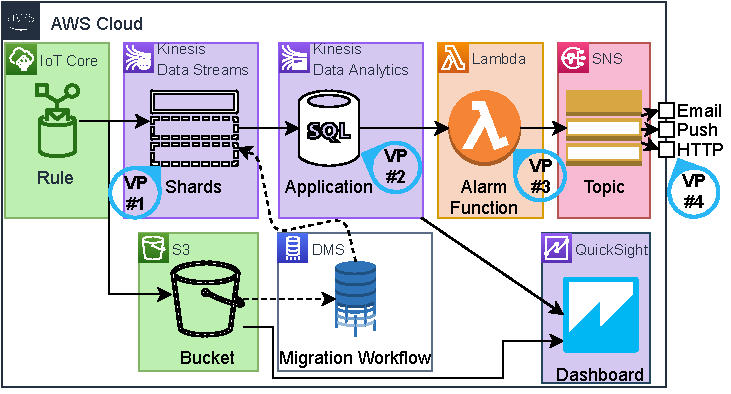
\includegraphics[width=\textwidth]{graphics/Echtzeit-RA-Elements.pdf}
\caption{Bausteinsicht mit Data Streams}
\label{abb:ElementeEchtzeitRAStreams}
\end{figure}
\textbf{Variationspunkte G3, G4, G5}: Siehe oben: \vpref{G3}, \vpref{G4}, \vpref{G5}

\vp{C1}: Die Anzahl an Shards ist essentiell für die Performance von Kinesis Data Streams. Für Workloads mit einem vorhersehbaren Workload ist Anzahl an Shards nach einem Preis/Leistungs Optimum zu ermitteln und zu konfigurieren. Wenn der Workload nicht vorhersehbar ist oder schnell skalieren können soll, sind Alarme im AWS eigenen Monitoring Tool CloudWatch zu erstellen. Im Beispielusecase für die Kostenschätzung ist ein einziger Shard (1MiB/Sekunde, 1000 Nachrichten eingehend) ausreichend. Dies ist bedingt, da Nachrichten mit einer Größe von 1KB, also ca. 1KiB geschrieben werden, bei einem Maximum von 200 pro Sekunde und einem Konsumenten. Es ist besonders auf die \enquote{WriteProvisionedThroughputExceeded} Metrik zu achten, welche bei höheren Werten anzeigt, dass das Hinzufügen von zusätzlichen Shards angebracht wäre. Ebenfalls ist die Metrik \enquote{Incoming Records} zu beachten. Verändert diese sich, deutet das auf einen Fehler im vorgelagerten \AWSIOT{} Core oder in einem Teil der Datenlieferanten hin.

\subsection{Anforderungen}
Folgend wird die Anwendbarkeit der Referenzarchitektur auf die definierten Anforderungen dargestellt.

\miniabschnitt{Anwendbarkeit auf Monitoringdaten (IT)}
Kinesis als System ist gut auf diverse Zeitseriendaten anwendbar. Problematisch ist das eigene Übertragungsformat, welches von Datenproduzenten verlangt, spezielle Schnittstellen zu implementieren. Der von \ac{AWS} vorgesehene Weg, die Kinesis Producer Library ist in Java geschrieben und bindet eine ausführbare C\texttt{++} Datei ein.\footcite[Vgl.][]{AmazonWebServicesInc..o.J.bg} Im Einsatz mit Monitoringdaten würde dies erfordern, dass die Daten in einem Standardformat aggregiert und dann mittels eines in Java geschriebenen Programms transformiert werden müsste. 

CloudWatch bietet diese Funktionalität mittels der CloudWatch Metric Streams und der CloudWatch Log Subscriptions an.\footcite[Vgl. auch im Folgenden][]{Barr.2021} Bei Metric Streams werden Metriken auf Wunsch in das OpenTelemetry oder das \ac{JSON} Format konvertiert und dann an Kinesis Data Firehose zur Weiterverarbeitung übermittelt. Dabei werden aber nur Metriken erfasst, die einen Zeitstempel jünger als zwei Stunden haben, was manche Metriken, die einmal am Tag versendet werden ausschließt. Zusätzlich muss ein Metric Stream in jeder Region angelegt werden, wo CloudWatch Logs anfallen, was eine Herausforderung in stark verteilten \ac{AWS}-Accounts darstellen kann. Metric Streams kosten 0,003\$ pro 1000 verarbeitete Metriken und zusätzlich die entsprechend anfallenden Data Firehose Gebühren. CloudWatch Log Subscriptions bietet sowohl streaming an Kinesis Data Streams, als auch an Kinesis Data Firehose an.\footcite[Vgl. auch im Folgenden][]{AmazonWebServicesInc..o.J.bk} Für jede Loggruppe, die einem Dienst oder einer einzelnen Ressource, wie beispielsweise einer Lambdafunktion zugeordnet sein kann, ist eine Subscription zu erstellen. Um dies zu erleichtern, sollte von Infrastructure as Code Gebrauch gemacht werden, um die Subscription automatisch für jede erstellte Loggruppe einzurichten. Es können benutzerdefinierte Filter eingerichtet werden, um nur relevante Logs zu übermitteln.

Insgesamt scheint die Kinesis Dienstfamilie gut geeignet, um sowohl Logs als besondere Zeitreihendaten, als auch Metriken skalierbar zu verarbeiten.

\miniabschnitt{Anwendbarkeit auf Sensordaten (IoT)}
Kinesis ist generalisiert ausgelegt, durch die Integration mit \AWSIOT{} Core wird jedoch die Verarbeitung von \ac{IoT} Daten einfach ermöglicht. Durch die schnelle Verarbeitung, die durch die Verwendung von Diensten aus der Kinesis Familie gewährleistet ist, können Analysen Ereignisse schnell aufzeigen. So ist, wie in \anhangref{anhang:interview-peter-24.03.2021} und \anhangref{anhang:interview-ralph-24.03.2021} erläutert, ein wesentlicher Teil der Erkenntnisse, die aus \ac{IoT}-Daten gewonnen werden können nur für einen kurzen Zeitraum relevant. Dies deckt sich mit der in \autoref{chap:datenwert} gezeigten Theorie der Datenhalbwertszeit und speziell dem taktischen Entscheidertypen, für den der Wert der Daten schnell abnimmt. Speziell wenn Aktionen folgend auf ein Ereignis ausgelöst werden sollen, ist deshalb eine schnelle Zeit bis zur Auswertung wichtig.

\miniabschnitt{Handling von Events, Messwerten und \enquote{Streaming}}
Da die Verarbeitungslogik in Kinesis Data Analytics selbst zu schreiben ist, ist die unterschiedliche Behandlung von Events, niedrigfrequenten Messwerten und Streaming implementierungsabhängig. Dabei wäre es zu empfehlen ein Attribut in die übermittelten Nachrichten einzufügen, welches den geanauen Typ der Nachricht definiert und entsprechende Verarbeitungslogiken vereinfacht. Zu diesem Zweck soll das Attribut \mintinline[breaklines]{json}{{"messageType": "<string>"}} dienen. Für Events, die Definitionsgemäß keinen Messwert beinhalten, ist das Attribut mit dem Wert \mintinline[breaklines]{json}{{"messageType": "event"}} zu belegen. Messwerte sollen \mintinline[breaklines]{json}{{"messageType": "meas_low_freq"}} als Wert verwenden. Für hochfrequentes Streaming ist \mintinline[breaklines]{json}{{"messageType": "meas_high_freq"}} zu verwenden.

\miniabschnitt{Automatisierte operative Entscheidungen}
Automatisierte Entscheidungen bzw. Handlungen sind mit Kinesis Data Analytics möglich. So könnte die selbe Lambdafunktion, die für die Alarmierung benutzt wird, auch Aktionen auslösen. Vorstellbar wäre, dass die Lambdafunktion über \ac{MQTT} Aktoren ansteuert, weitere Akteure informiert (z.B. die Werksfeuerwehr) oder selbstständig Anweisungen auslöst, die den Alarm beheben (so könnte bei niedrigem Batteriestand eine neue Batterie für einen Sensor geordert werden). 


\subsection{Produktives Monitoringkonzept} \label{chap:echtzeit_ops}
Um den Betrieb der instanziierenden Architekturen zu sichern, wird folgend ein Monitoringkonzept dargestellt, welches die zu überwachenden Metriken der verwendeten Dienste zeigt. So soll verhindert werden, dass der Datenwert durch Analyse nicht genutzt werden kann, weil ein Infrastrukturproblem besteht.
In \autoref{tab:cloudwatch-metrics-rt} werden Kinesis Data Streams, \ac{SNS}, \AWSIOT{} Core, Kinesis Data Analytics und Kinesis Data Firehose betrachtet.\footcite[Vgl.][]{AmazonWebServicesInc..o.J.bb}\nzitat\footcite[Vgl.][]{AmazonWebServicesInc..o.J.bc}\nzitat\footcite[Vgl.][]{AmazonWebServicesInc..o.J.az}\nzitat\footcite[Vgl.][]{AmazonWebServicesInc..o.J.ay}\nzitat\footcite[Vgl.][]{AmazonWebServicesInc..o.J.bj}

\begin{table}[H]
\centering
\begin{tabular}{|l|l|l|l|}
\hline
Dienst & Metrik & Ursache & Detektionsart \\ \hline
\rowcolor[HTML]{F5F5F5} 
\ac{SNS} & NumberOfNotificationsFailed & Dienstfehler & Schwellwert \\ \hline
 & RuleMessageThrottled & Dienstfehler & Schwellwert \\ \cline{2-4} 
\multirow{-2}{*}{\AWSIOT{} Core} & Failure & \begin{tabular}[c]{@{}l@{}}Dienstfehler/\\ Benutzungsfehler\end{tabular} & Schwellwert \\ \hline
\rowcolor[HTML]{F5F5F5} 
\cellcolor[HTML]{F5F5F5} & MillisBehindLatest & \begin{tabular}[c]{@{}l@{}}Dienstfehler/\\ Benutzungsfehler\end{tabular} & Anomalie \\ \cline{2-4} 
\rowcolor[HTML]{F5F5F5} 
\cellcolor[HTML]{F5F5F5} & LambdaDelivery.DeliveryFailedRecords & \begin{tabular}[c]{@{}l@{}}Dienstfehler/\\ Benutzungsfehler\end{tabular} & Schwellwert \\ \cline{2-4} 
\rowcolor[HTML]{F5F5F5} 
\multirow{-3}{*}{\cellcolor[HTML]{F5F5F5}\begin{tabular}[c]{@{}l@{}}Kinesis \\ Data Analytics\end{tabular}} & LambdaDelivery.Duration & \begin{tabular}[c]{@{}l@{}}Dienstfehler/\\ Benutzungsfehler\end{tabular} & Anomalie \\ \hline
 & WriteProvisionedThroughputExceeded & Benutzungsfehler & Schwellwert \\ \cline{2-4} 
 & ReadProvisionedThroughputExceeded & Benutzungsfehler & Schwellwert \\ \cline{2-4} 
 & GetRecords.Latency & Dienstfehler & Anomalie \\ \cline{2-4} 
\multirow{-4}{*}{\begin{tabular}[c]{@{}l@{}}Kinesis \\ Data Streams \\ (VP G1)\end{tabular}} & PutRecords.ThrottledRecords & \begin{tabular}[c]{@{}l@{}}Dienstfehler/\\ Benutzungsfehler\end{tabular} & Schwellwert \\ \hline
\rowcolor[HTML]{F5F5F5} 
\cellcolor[HTML]{F5F5F5} & \begin{tabular}[c]{@{}l@{}}DeliveryToS3.Records/ \\ DeliveryToS3.Success (Verhältnis)\end{tabular} & Dienstfehler & Schwellwert \\ \cline{2-4} 
\rowcolor[HTML]{F5F5F5} 
\cellcolor[HTML]{F5F5F5} & ThrottledRecords & Dienstfehler & Schwellwert \\ \cline{2-4} 
\rowcolor[HTML]{F5F5F5} 
\multirow{-3}{*}{\cellcolor[HTML]{F5F5F5}\begin{tabular}[c]{@{}l@{}}Kinesis \\ Data Firehose \\ (VP G1)\end{tabular}} & PutRecord.Latency & Dienstfehler & Anomalie \\ \hline
\end{tabular}
\caption{CloudWatch Metriken}
\label{tab:cloudwatch-metrics-rt}
\end{table}
Die Metriken werden von Kinesis einmal pro Minute an CloudWatch übermittelt.\footcite[Vgl. auch im Folgenden][]{Pogosova.28.05.2020} Dies birgt die Gefahr, bei nicht konstanten Workloads, dass erst mit Verzögerung gehandelt werden kann. Bei besonders wechselhafter Last sollte also davon ausgegangen werden, dass nicht die tatsächliche Spitzenlast bekannt ist, sondern mit einem Aufschlag gearbeitet werden muss. 

Unterschieden wird in der Tabelle zwischen Fehlern, die auf den Dienst zurückzuführen sind und Fehlern, die durch Falschbedienung der Nutzenden entstehen können. Es ist auch möglich, dass Fehler durch mehrere verknüpfte Dienste kaskadieren und mehrere Metriken Alarme auslösen. Dies wäre beispielsweise der Fall, wenn sehr schnell viel mehr Nachrichten als im Normalzustand eingehen. Ausgehend von der Spalte Detektionsart können Alarme in CloudWatch aufgesetzt werden.


\subsection{Know-how für instanziierende Architekturen}
Folgend wird die Möglichkeit zum Autoscaling bei Kinesis Data Streams und die genaue Übermittlungssemantik beim Einsatz mit \AWSIOT{} Core addressiert als Themen, die besonderer Aufmerksamkeit bei der Instanziierung bedürfen.

\miniabschnitt{Autoscaling bei Kinesis Data Analytics}
Wie bereits beschrieben, bietet Kinesis Data Streams keine automatisierte Skalierung der Shards an. Da es durchaus, wie in \vpref{G1} geschildert, Einsatzszenarien für Kinesis Data Streams gibt, sollen folgend die diversen Ansätze für Autoscaling bei Kinesis Data Streams aufgezeigt werden. Dies soll, im Fall dass Kinesis Data Streams eingesetzt wird, dabei helfen, Kinesis Data Streams skalierend zu betreiben. Dieses Problem wurde durch die Gemeinschaft aus Nutzenden und Programmierenden in vielerlei Art adressiert. 
Der von \citeauthor{AmazonWebServices.2018} vorgestellte, \ac{AWS} eigene Ansatz basiert auf CloudWatch Alarmen, die basierend auf den IncomingBytes und IncomingRecords Shards eine Lambda auslösen, welche die Skalierung verwaltet.\footcite[Vgl.][]{AmazonWebServices.2018}\nzitat\footnote{Siehe auch: \url{https://github.com/aws-samples/aws-application-auto-scaling-kinesis}} 
\citeauthor{Pogosova.28.05.2020} kritisert, dass die Menge von fünf Diensten, die diese Lösung benötigt, kaum als autoscaling zu bezeichnen ist.\footcite[Vgl.][]{Pogosova.28.05.2020} 
\citeauthor{Stanley.2019} schlägt zur Lösung des Problems eine Lösung und eine Beispielimplementation in Python vor, die ebenfalls auf CloudWatch Alarmen basiert, aber eine \ac{MoM} zwischenschaltet, die dann eine Lambdafunktion ausführt.\footcite[Vgl.][]{Stanley.2019} 
\citeauthor{Prasath.2019} setzt auf einen vergleichbaren Ansatz wie \citeauthor{Stanley.2019}, nur dass keine konkrete Implementierung vorgeschlagen wird.\footcite[Vgl.][]{Prasath.2019} 
\citeauthor{Cui.2017} modifiziert den Ansatz unter Berücksichtigung des Faktes, dass das herunterskalieren von Shards teurer sein könnte, wenn der Datendurchsatz nicht genau bekannt ist.\footcite[Vgl. auch im Folgendn][]{Cui.2017} Zur Mitigation schlägt \citeauthor{Cui.2017} eine Herunterskalierung durch einen CloudWatch Auslöser vor, der erst 36h später auslöst. 

Allen Ansätzen zueigen ist, dass eine Verzögerung wie in \autoref{chap:echtzeit_ops} geschildert, von 60 Sekunden bis zur Erfassung der aktuellen Metriken besteht. Dies birgt die Gefahr, dass für eine gewisse Zeit zu wenige Shards provisioniert sind. Aufgrund der Komplexität, ein passendes Autoscaling zu errichten ist es angezeigt, wenn die Performance von Data Firehose in Tests ausreicht, Data Firehose entsprechend dem \vpref{G1} zu verwenden.

\miniabschnitt{Idempotenz bei Auswertungen}
Zu beachten ist in allem Analysecode die Möglichkeit, dass Nachrichten doppelt auftreten und die Auswertungsergebnisse verfälschen. Folgend wird auf die \textit{exactly-once} Semantik eingegangen und ob diese in der Referenzarchitektur verfügbar ist.
Innerhalb des MQTT Protkolls, das \AWSIOT{} Core in Teilen implementiert ist für die zwei  \ac{QoS} Modi 0 und 1 eine \textit{at-least-once} Semantik vorgesehen.\footcite[Vgl. auch im Folgenden][]{OASISOpenConsortium.2014} Der \ac{QoS} Modus 2, welcher eine \textit{exactly-once} Semantik garantiert, wird von \AWSIOT{} Core nicht unterstützt.\footcite[Vgl.][]{AmazonWebServicesInc..o.J.bd} Zusätzlich ist eine \textit{exactly-once} Semantik bei der Ausführung von \AWSIOT{} Core Rules nicht garantiert. Wenn doppelte Werte für Auswertungen nicht tolerierbar sind, muss entsprechend eine Deduplizierung eingeführt werden. 

Aufgrund des technischen Aufwandes, der hinter einer Deduplizierung und garantierter Idempotenz steht, muss genau abgewogen werden, ob die fachlichen Seite des Anwendungsfalls eine doppelte Verarbeitung mancher Records nicht tolerieren kann. So wäre beispielsweise ein doppelter Messwert, der eine Überschreitung anzeigt wenig kritisch. Bei Aggregationen wie dem gleitenden Durchschnitt verringert der Einfluss eines einzelnen doppelten Wertes eines Sensors sich mit wachsender Anzahl $n$ der angeschlossenen Sensoren. Eine mögliche Mitigation wäre, die Messzeit zusammen mit den Messwerten zur Deduplikation zu verwenden. Dabei ist zu beachten, dass die Möglichkeit besteht, dass die integrierte Uhr des Sensors falsch geht.